% chktex-file 44
% chktex-file 1

\section{\large  Ejercicio 5. Sistemas de Ecuaciones con infinitas soluciones}

Cada uno de los siguientes sistemas de ecuaciones lineales homogéneo $(2\times3)$, tiene infinitas soluciones. Para cada sistema, realiza lo siguiente:

\[
    C=
    \begin{cases}
        \begin{aligned}
            3x-5y+z=0 \\
            15x-25y+5y=0 \\
        \end{aligned}
    \end{cases}
\]

\begin{itemize}
    \item Determine el conjunto solución.
    \[
        \begin{aligned}
            \left(
                \begin{array}{ccc|c}
                    3 & -5 & 1 & 0 \\
                    15 & -25 & 5 & 0 \\
                \end{array}
            \right)
            &\frac{f1}{3} \\ \\
            \left(
                \begin{array}{ccc|c}
                    1 & -\frac{5}{3} & \frac{1}{3} & 0 \\
                    15 & -25 & 5 & 0 \\
                \end{array}
            \right)
            &-15f1+f2 \\ \\
            \begin{array}{ccc|c}
                -15 & \frac{75}{3} & -\frac{15}{3} & 0 \\
                15 & -25 & 5 & 0 \\
                \hline
                0 & 0 & 0 & 0
            \end{array} \\ \\
            \left(
                \begin{array}{ccc|c}
                    1 & -\frac{5}{3} & \frac{1}{3} & 0 \\
                    0 & 0 & 0 & 0 \\
                \end{array}
            \right) \\ \\
            x-\frac{5}{3}y+\frac{1}{3}z=0 \\ \\
            \left(
                1,-\frac{5}{3}y,\frac{1}{3}z
            \right)
        \end{aligned}
    \]
    \begin{figure}[ht!]
        \centering
        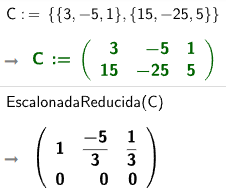
\includegraphics[width=140pt,height=100pt]{img/imagen13.png}
        \caption{Comprobación en GeoGebra}
    \end{figure}

    \item Identifique un sistema fundamental de soluciones, es decir, una base que genere el conjunto solución obtenido en el ítem anterior.
    \[
        \begin{aligned}
            x-\frac{5}{3}(1)+\frac{1}{3}(0)=0 \\
            x-\frac{5}{3}=0 \\
            x=\frac{5}{3} \\
        \end{aligned}
    \]
    \[
        \begin{aligned}
            x-\frac{5}{3}(2)+\frac{1}{3}(1)=0 \\
            x-\frac{10}{3}+\frac{1}{3}=0 \\
            x-\frac{9}{3}=0 \\
            x-3=0 \\
            x=3 \\ \\
        \end{aligned}
    \]
    \[
        \begin{aligned}
            x-\frac{5}{3}(3)+\frac{1}{3}(2)=0 \\
            x-\frac{15}{3}+\frac{2}{3}=0 \\
            x-5+\frac{2}{3}=0 \\
            x-\frac{13}{3}=0\\
            x=\frac{13}{3}
        \end{aligned}
    \]
    \[
        \begin{aligned}
            x-\frac{5}{3}(4)+\frac{1}{3}(3)=0 \\
            x-\frac{20}{3}+\frac{3}{3}=0 \\
            x-\frac{20}{3}+1=0 \\
            x-\frac{17}{3}=0 \\
            x=\frac{17}{3}
        \end{aligned}
    \]
    \[
        \left\{
            \left(
                \frac{5}{3},1,0
            \right),
            \left(
                3,2,1
            \right),
            \left(
                \frac{13}{3},3,2
            \right),
            \left(
                \frac{17}{3},4,3
            \right)
        \right\}
    \]
    \begin{figure}[ht!]
        \centering
        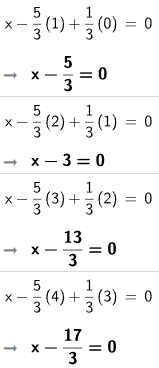
\includegraphics[width=140pt,height=400pt]{img/imagen14.png}
        \caption{Comprobación en GeoGebra}
    \end{figure}

    \item Describa la naturaleza geométrica de la solución obtenida en el ítem anterior (si corresponde a una recta o un plano en el espacio). Puede utilizar GeoGebra para realizar una verificación geométrica visual de la solución.
    \begin{figure}[ht!]
        \centering
        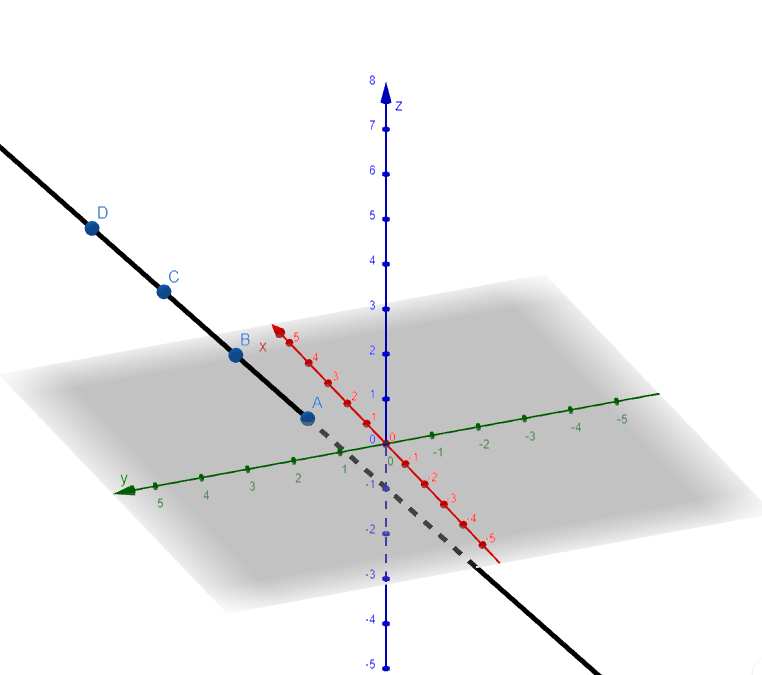
\includegraphics[width=400pt,height=400pt]{img/imagen15.png}
        \caption{Graficación de los puntos en GeoGebra}
    \end{figure}
    \FloatBarrier
    \begin{center}
        \textit{\textbf{Solución: }Como se puede ver en la gráfica de GeoGebra, la naturaleza geométrica de la solución obtenida es una recta.}
    \end{center}
\end{itemize}